
%(BEGIN_QUESTION)
% Copyright 2011, Tony R. Kuphaldt, released under the Creative Commons Attribution License (v 1.0)
% This means you may do almost anything with this work of mine, so long as you give me proper credit

An analyzer used to measure the concentration of sulfur dioxide (SO$_{2}$) in the exhaust gas released out the smoke-stack of a large combustion furnace requires that the temperature of its sensor be precisely controlled.  The sensor temperature in this particular analyzer is controlled by an analog electronic controller circuit built out of op-amps.  Temperature is measured using a negative-coefficient thermistor (1500 ohms at room temperature, with resistance decreasing as temperature increases).  Heat is added to the analyzer's sensor enclosure by a 75 watt electric heating element controlled by the analog circuit:

$$\includegraphics[width=15.5cm]{i02910x01.eps}$$

After years of faithful service, it is determined that the lifespan of the (expensive) analytical sensor may be greatly increased by operating it at a lower temperature, without sacrificing its ability to accurately measure SO$_{2}$ gas concentration.  You are asked to decrease the setpoint of the analog temperature controller, but are dismayed to find the controller is entirely non-adjustable!  Not only is there no setpoint adjustment, but all the controller's components are ``potted'' in an impenetrable epoxy substance which means you cannot change any of the circuit board components (e.g. resistors, capacitors) to alter its setpoint.

\vskip 10pt

Devise a solution for making this temperature control system operate at a lower temperature, while still maintaining full ability to compensate for changes in ambient temperature.  Be as detailed in your explanation as necessary to describe your solution to the problem.

\underbar{file i02910}
%(END_QUESTION)





%(BEGIN_ANSWER)

A full-credit answer is one that will work under all conditions, while a half-credit answer is one that will only work under some conditions.

\vskip 10pt

Full-credit example: an explanation showing how to modify the thermistor circuit so that it registers a lesser resistance at the same temperature as before (therefore making the controller ``think'' the enclosure is too hot, causing it to regulate temperature at a lower effective setpoint).

Half-credit example: suggesting the heating element be handicapped (e.g. opening a vent on the enclosure, inserting resistance in series with the element) should only receive half-credit because while this may initially lower the operating temperature, the controller will eventually compensate.

Half-credit example: suggesting the thermistor be swapped for a different type, without specifying anything about the new thermistor (i.e. that it needs to have a lower resistance at any given temperature than the old thermistor).

%(END_ANSWER)





%(BEGIN_NOTES)

{\bf This question is intended for exams only and not worksheets!}

%(END_NOTES)


